%-----------------------------------------------------------------------------------------------------------------------------------------------%
%	The MIT License (MIT)
%
%	Copyright (c) 2021 Jitin Nair
%
%	Permission is hereby granted, free of charge, to any person obtaining a copy
%	of this software and associated documentation files (the "Software"), to deal
%	in the Software without restriction, including without limitation the rights
%	to use, copy, modify, merge, publish, distribute, sublicense, and/or sell
%	copies of the Software, and to permit persons to whom the Software is
%	furnished to do so, subject to the following conditions:
%	
%	THE SOFTWARE IS PROVIDED "AS IS", WITHOUT WARRANTY OF ANY KIND, EXPRESS OR
%	IMPLIED, INCLUDING BUT NOT LIMITED TO THE WARRANTIES OF MERCHANTABILITY,
%	FITNESS FOR A PARTICULAR PURPOSE AND NONINFRINGEMENT. IN NO EVENT SHALL THE
%	AUTHORS OR COPYRIGHT HOLDERS BE LIABLE FOR ANY CLAIM, DAMAGES OR OTHER
%	LIABILITY, WHETHER IN AN ACTION OF CONTRACT, TORT OR OTHERWISE, ARISING FROM,
%	OUT OF OR IN CONNECTION WITH THE SOFTWARE OR THE USE OR OTHER DEALINGS IN
%	THE SOFTWARE.
%	
%
%-----------------------------------------------------------------------------------------------------------------------------------------------%

%----------------------------------------------------------------------------------------
%	DOCUMENT DEFINITION
%----------------------------------------------------------------------------------------

% article class because we want to fully customize the page and not use a cv template
\documentclass[a4paper,12pt]{article}

%----------------------------------------------------------------------------------------
%	FONT
%----------------------------------------------------------------------------------------

% % fontspec allows you to use TTF/OTF fonts directly
% \usepackage{fontspec}
% \defaultfontfeatures{Ligatures=TeX}

% % modified for ShareLaTeX use
% \setmainfont[
% SmallCapsFont = Fontin-SmallCaps.otf,
% BoldFont = Fontin-Bold.otf,
% ItalicFont = Fontin-Italic.otf
% ]
% {Fontin.otf}

%----------------------------------------------------------------------------------------
%	PACKAGES
%----------------------------------------------------------------------------------------
\usepackage[utf8]{inputenc}
\usepackage[T2A]{fontenc}
\usepackage[russian,english]{babel}
\usepackage{url}
\usepackage{parskip} 	

%other packages for formatting
\RequirePackage{color}
\RequirePackage{graphicx}
\usepackage[usenames,dvipsnames]{xcolor}
\usepackage[scale=0.9]{geometry}

%tabularx environment
\usepackage{tabularx}

%for lists within experience section
\usepackage{enumitem}

% centered version of 'X' col. type
\newcolumntype{C}{>{\centering\arraybackslash}X} 

%to prevent spillover of tabular into next pages
\usepackage{supertabular}
\usepackage{tabularx}
\newlength{\fullcollw}
\setlength{\fullcollw}{0.47\textwidth}

%custom \section
\usepackage{titlesec}				
\usepackage{multicol}
\usepackage{multirow}

%CV Sections inspired by: 
%http://stefano.italians.nl/archives/26
\titleformat{\section}{\large\scshape\raggedright}{}{0em}{}[\titlerule]
\titlespacing{\section}{0pt}{6pt}{6pt}

%for publications
\usepackage[style=authoryear,sorting=ynt, maxbibnames=2]{biblatex}

%Setup hyperref package, and colours for links
\usepackage[unicode, draft=false]{hyperref}
\definecolor{linkcolour}{rgb}{0,0.2,0.6}
\hypersetup{colorlinks,breaklinks,urlcolor=linkcolour,linkcolor=linkcolour}
\addbibresource{citations.bib}
\setlength\bibitemsep{1em}

%for social icons
\usepackage{fontawesome5}

%debug page outer frames
%\usepackage{showframe}


% job listing environments
\newenvironment{jobshort}[2]
    {
    \begin{tabularx}{\linewidth}{@{}l X r@{}}
    \textbf{#1} & \hfill &  #2 \\[3.75pt]
    \end{tabularx}
    }
    {
    }

\newenvironment{joblong}[2]
    {
    \begin{tabularx}{\linewidth}{@{}l X r@{}}
    \textbf{#1} & \hfill &  #2 \\[3.75pt]
    \end{tabularx}
    \begin{minipage}[t]{\linewidth}
    \begin{itemize}[nosep,after=\strut, leftmargin=1em, itemsep=3pt,label=--]
    }
    {
    \end{itemize}
    \end{minipage}    
    }



%----------------------------------------------------------------------------------------
%	BEGIN DOCUMENT
%----------------------------------------------------------------------------------------
\begin{document}

% non-numbered pages
\pagestyle{empty} 

%----------------------------------------------------------------------------------------
%	TITLE
%----------------------------------------------------------------------------------------

% \begin{tabularx}{\linewidth}{ @{}X X@{} }
% \huge{Your Name}\vspace{2pt} & \hfill \emoji{incoming-envelope} email@email.com \\
% \raisebox{-0.05\height}\faGithub\ username \ | \
% \raisebox{-0.00\height}\faLinkedin\ username \ | \ \raisebox{-0.05\height}\faGlobe \ mysite.com  & \hfill \emoji{calling} number
% \end{tabularx}

\begin{tabularx}{\linewidth}{@{} C @{}}
\LARGE{Якупов Самат | Frontend Developer} \\[4pt]
\small{\href{https://github.com/samerspc}{\raisebox{-0.05\height}\faGithub\ samerspc} \ $|$ \  
\href{https://t.me/samerspc}{\raisebox{-0.05\height}\faTelegram \ samerspc} \ $|$ \ 
\href{sa.iakupov@innopolis.university}{\raisebox{-0.05\height}\faEnvelope \ sa.iakupov@innopolis.university} \ $|$ \ 
\href{tel:+79695331993}{\raisebox{-0.05\height}\faMobile \ +7 (969) 533-19-93}} \\
\end{tabularx}\\[6pt]

%----------------------------------------------------------------------------------------
% EXPERIENCE SECTIONS
%----------------------------------------------------------------------------------------

%Interests/ Keywords/ Summary
\section{Технологии}

\begin{tabularx}{\linewidth}{@{}l X@{}}
\textbf{ЯП и фреймворки} & \small{JavaScript (ES6+), TypeScript, React} \\[1pt]
\textbf{Состояние/данные} & \small{Redux Toolkit, React Query, RTK Query} \\[1pt]
\textbf{Вёрстка/стили} & \small{HTML5, CSS3, SCSS/SASS, CSS-Modules, Tailwind CSS} \\[1pt]
\textbf{Тесты} & \small{Jest, Cypress} \\[1pt]
\textbf{Сборка/инфра} & \small{Vite/Webpack, GitHub Actions, Docker, Node.js, Yandex Cloud S3, CDN} \\[1pt]
\textbf{Деплой/CI/CD} & \small{GitHub Actions, автодеплой, Docker-контейнеры, Vercel/Netlify} \\[1pt]
\textbf{Инструменты} & \small{REST, GraphQL, WebSockets, Figma, ESLint, Prettier, Storybook} \\
\end{tabularx}
\\[6pt]
% Projects
\section{Проекты}

\begin{tabularx}{\linewidth}{ @{}l r@{} }
\textbf{Stellar Burgers — React, TypeScript, Redux Toolkit, Router} & \hfill \href{https://github.com/samerspc/yandex-practicum__stellar-burgers}{GitHub} \\[-8pt]
\multicolumn{2}{@{}X@{}}{
\begin{itemize}[nosep,after=\strut, leftmargin=1em, itemsep=2pt,label=--]
\item Реализовал полную авторизацию (регистрация/логин/восстановление), защищённые маршруты и профиль пользователя
\item Организовал глобальное состояние на Redux Toolkit с thunk-функциями; выделил слои services/hooks/store
\item Собрал UI-конструктор бургеров с drag\&drop, модалками и маршрутизацией; оформил компоненты в Storybook
\end{itemize}
}  \\
\end{tabularx}

% \vspace{4pt}

\begin{tabularx}{\linewidth}{ @{}l r@{} }
\textbf{nitted.shop — full-stack интернет-магазин} & \hfill \href{https://github.com/samerspc/nitted.shop}{GitHub} \\[-8pt]
\multicolumn{2}{@{}X@{}}{
\begin{itemize}[nosep,after=\strut, leftmargin=1em, itemsep=2pt,label=--]
\item Собрал каталог, фильтры и карточки товара; сделал админ-панель для управления контентом
\item Организовал хранение изображений в \textbf{Yandex Cloud Object Storage (S3)}: прямой upload с фронта по presigned URL
\item Подключил отправку заявок через Telegram Bot API; описал простые API-контракты и валидацию
\item Настроил CD: автосборка и деплой на сервер из репозитория; вёрстка по Figma, адаптив и кроссбраузерность
\end{itemize}
}  \\
\end{tabularx}

\vspace{4pt}

\begin{tabularx}{\linewidth}{ @{}l r@{} }
\textbf{Collaborative Editor — онлайн-канвас (STOMP/WebSockets)} & \hfill \href{https://github.com/samerspc/collaborative_editor}{GitHub} \\[-8pt]
\multicolumn{2}{@{}X@{}}{
\begin{itemize}[nosep,after=\strut, leftmargin=1em, itemsep=2pt,label=--]
\item Реализовал многопользовательские сессии и комнаты с синхронизацией событий через STOMP
\item Обработал реконнекты и консистентность состояния на клиенте; выделил слой обмена сообщениями
\item Сделал инструменты канваса (кисть/цвет/толщина), горячие клавиши и доступные модалки
\end{itemize}
}  \\
\end{tabularx}

%Experience
\section{Опыт}

\begin{joblong}{JavaScript-разработчик (частичная занятость) — learnthemap.com}{08.2024–12.2024}
\item Верстал адаптивные страницы по Figma макетам
\item Исправлял баги вёрстки и JS, участвовал в код-ревью
\end{joblong}

%----------------------------------------------------------------------------------------
%	EDUCATION
%----------------------------------------------------------------------------------------
\section{Образование}
\begin{tabularx}{\linewidth}{@{}l X@{}}	
2024 - 2027 & Бакалавр, «Инженерия информационных систем» в \textbf{Университет Иннополис} \hfill \small{3 курс} \\
2025 & Курс «Фронтенд-разработчик» в \textbf{Яндекс Практикум} \\
\end{tabularx}

%----------------------------------------------------------------------------------------
%	ADDITIONAL INFO
%----------------------------------------------------------------------------------------
\section{Дополнительно}
\begin{tabularx}{\linewidth}{@{}l X@{}}
\textbf{Языки} & \small{RU — родной, EN — B2-C1 (сертификат)} \\[2pt]
\textbf{ATS keywords} & \small{React, TypeScript, Redux Toolkit, Jest, Cypress, REST, GraphQL, WebSockets, GitHub Actions} \\
\end{tabularx}

%----------------------------------------------------------------------------------------
%	CERTIFICATE
%----------------------------------------------------------------------------------------
\section{Сертификаты}
\begin{center}
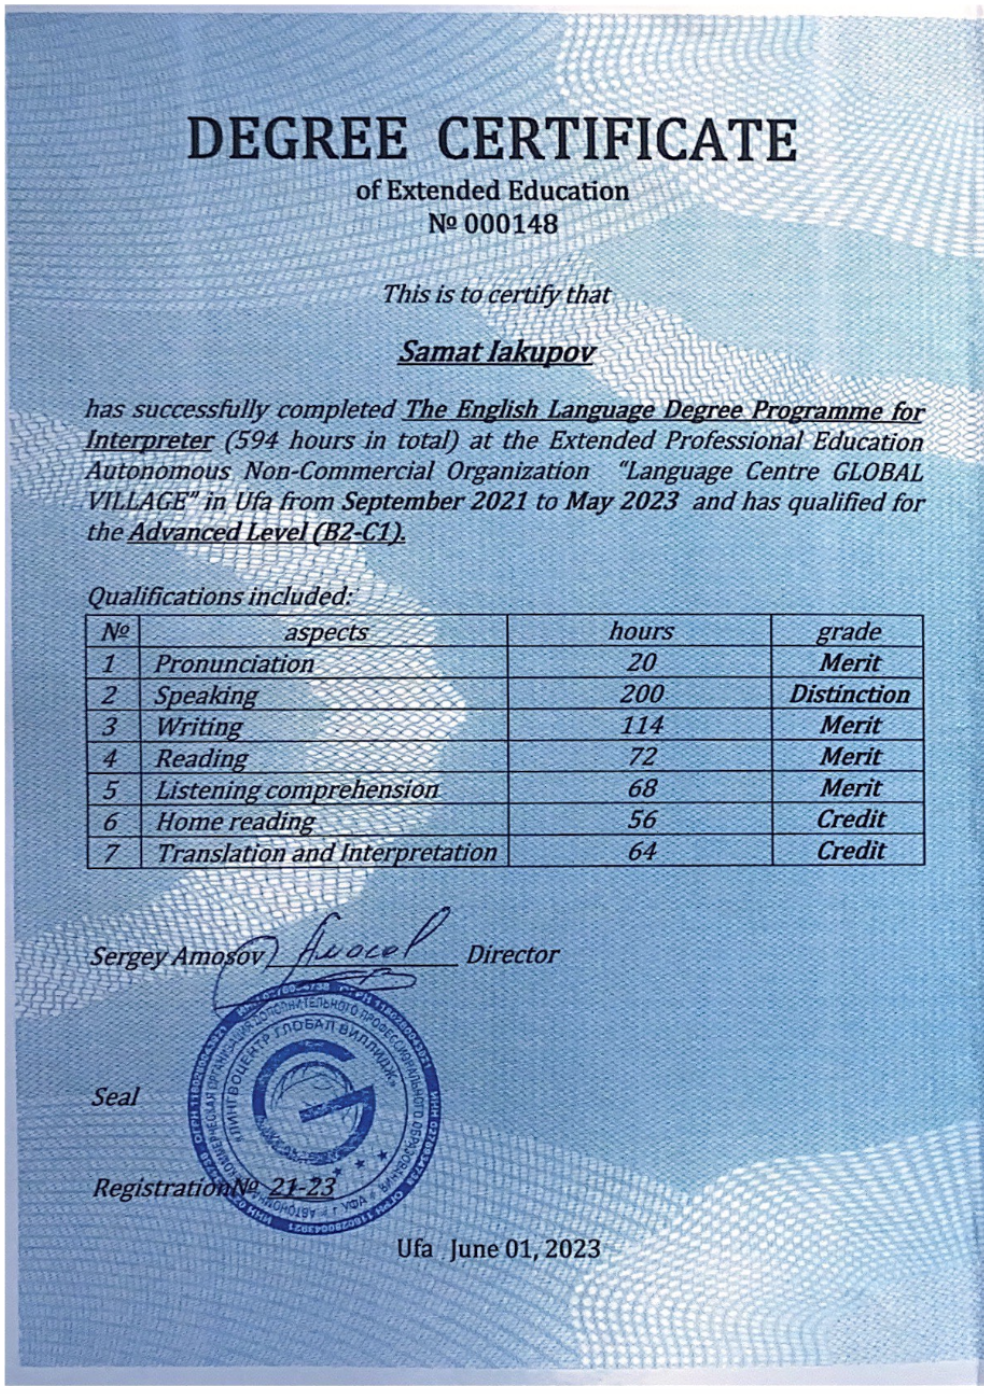
\includegraphics[width=0.65\textwidth]{cert.png}
\end{center}

\vfill
\center{\footnotesize Last updated: \today}

\end{document}
